%%%%%%%%%%%%%%%%%%%%%%%%%%%%%%%%%%%%%%%%%%%%%%%%%%%%%%%%%%%%%%%%%%
%%%%%%%%%%%%%%%%%%%%%%%%%%%%%%%%%%%%%%%%%%%%%%%%%%%%%%%%%%%%%%%%%%
%% 
%%     S E C T I O N    4         S E C T I O N    4           S E C T I O N    4       S E C T I O N   4
%%     S E C T I O N    4         S E C T I O N    4           S E C T I O N    4       S E C T I O N   4
%%     S E C T I O N    4         S E C T I O N    4           S E C T I O N    4       S E C T I O N   4
%%
%%%%%%%%%%%%%%%%%%%%%%%%%%%%%%%%%%%%%%%%%%%%%%%%%%%%%%%%%%%%%%%%%%
%%%%%%%%%%%%%%%%%%%%%%%%%%%%%%%%%%%%%%%%%%%%%%%%%%%%%%%%%%%%%%%%%%
\section{Surface Density of VH$z$Qs}
One interesting question to ask is given the compilation of VH$z$Qs assembled here, 
are there bright $z>5.00$ quasars that are in {\it current} photometric datasets, and if 
so, how many are still to be discovered and confirmed spectroscopically?

In the North, we assume the UHS J-band depth of 19.6 \citep[Vega;
][]{Dye2018}.  In the South, one can use the report {\tt ABmagLimits}
for each survey in the database, we can calculate the depths of the
various NIR VISTA surveys.  Fig.~\ref{fig:VHS_J_abMagLim} shows this
calculated average {\tt AB MAGLIM} in the VHS.  As one can see, the
VHS is not completely uniform. The area wrapping round
310$\lesssim$RA/deg$\lesssim$90 and -70$\lesssim$ Decl./ deg
$\lesssim$ -40 has a $J$-band depth of 21.2 AB mag, whereas the rest
of the VHS area, the $J$-band depth is closer to 20.6 AB mag.

\begin{figure}
  \centering
  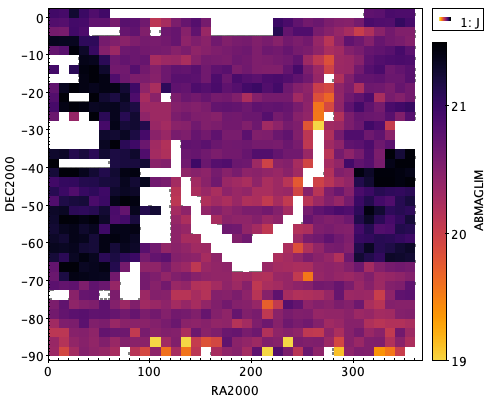
\includegraphics[width=8.5cm]{../data/WSA_VSA/VHS_J_abMagLim.png}
  \caption{The calculated average {\tt AB MAGLIM} in the VHS.
    As one can see, VHS is not completely uniform. The are 3 areas with different filter sets, 
    and the depths changed in 2 of these areas, particularly in $J$ and $K_{s}$. 
    Y and H are almost uniform, but the coverage is much less.}
  \label{fig:VHS_J_abMagLim}
\end{figure}

Following \citet{Fan2001b} and \citet{McGreer2013}, we use use an
exponential decline to describe the space density of VH$z$Qs at high
redshifts, e.g.
\begin{equation}
\rho(z, {\rm M}_{1450}) \propto 10^{k (z)}
\end{equation}
where $z$ is the sample redshift. 
%Fan, X., Strauss, M. A., Schneider, D. P., et al. 2001b, AJ, 121, 54
